\documentclass{article}
\usepackage[utf8]{inputenc}
\usepackage{graphicx}
\usepackage[italian]{babel}
\usepackage{listings}
\usepackage{rest-api}
\usepackage{gRPC/lang}
\usepackage{gRPC/style}
\usepackage{enumitem}
\usepackage{courier}
\usepackage{minted}


\setcounter{secnumdepth}{4}
\setcounter{tocdepth}{4}


\title{
    
\includegraphics[width=0.5\textwidth]{img/unict-universita-di-catania.png}\\
    \bigskip
    \LARGE Corso di Distribuited System and Big Data\\
    A.A. 2022-2023\\
    \Huge Relazione progetto in itinere\\
    \bigskip
    \Large 
}
\author{Alessio Pirri (1000040385), Mattia Pirri (1000042320)}
\date{31 Gennaio 2023}

\begin{document}

\maketitle
\newpage
\tableofcontents
\newpage

\section{Abstract}
Si vuole realizzare un sistema distribuito per il monitoraggio di un'applicazione. L'applicazione espone già le metriche da monitorare tramite un server Prometheus. Vengono realizzati i seguenti microservizi: 
\begin{itemize}
    \item ETL data pipeline: esegue due loop in parallelo: 
        \begin{itemize}
            
            \item il primo con periodo di \textbf{2 min} che si occupa di calcolare i valori statistici di aggregazione e di effettuare la predizione dei successivi 10 minuti per le metriche dell'SLA set.
            \item il secondo con periodo di \textbf{1h} che si occupa di calcolare i metadati per ogni metrica esposta dal Prometheus
        \end{itemize}
        Entrambi i loop inoltrano i dati al topic kafka "prometheusdata". Vengono monitorati i tempi di esecuzione delle varie funzionalità mediante un exporter Prometheus.
    \item Data Storage: consumer kafka del topic "prometheusdata" che si occupa di scrivere i dati ricevuti dall'ETL data pipeline e di memorizzarli in un database MongoDB
    \item Data Retreival: interfaccia REST che permette di estrarre le informazioni contenute nel database.
    \item SLA Manager: microservizio che consente, tramite interfaccia REST la definizione dell'SLA set e la possibilità di sapere lo stato dell'SLA. Tramite interfaccia gRPC consente all'ETL data pipeline di ottenere l'SLA set. In fase di definizione dell'SLA set è possibile indicare 5 metriche e, per ognuna di esse, il range all'interno del quale il valore della metrica deve rimanere e il tempo necessario per far scattare l'allarme per la violazione.
\end{itemize}
Per il deploy del sistema si è utilizzato un \textbf{Docker Compose}. È stata effettuata anche una prova di deployment tramite l'orchestratore di container \textbf{Kubernetes}.
Le metriche scelte sono:
\begin{itemize}
    \item node\_filesystem\_avail\_bytes
    \item cpuTemp
    \item diskUsage
    \item realUsedMem
    \item networkTroughput
\end{itemize}
 \newpage
\section{Schema architetturale}
    \begin{figure}[h]
        \centering
        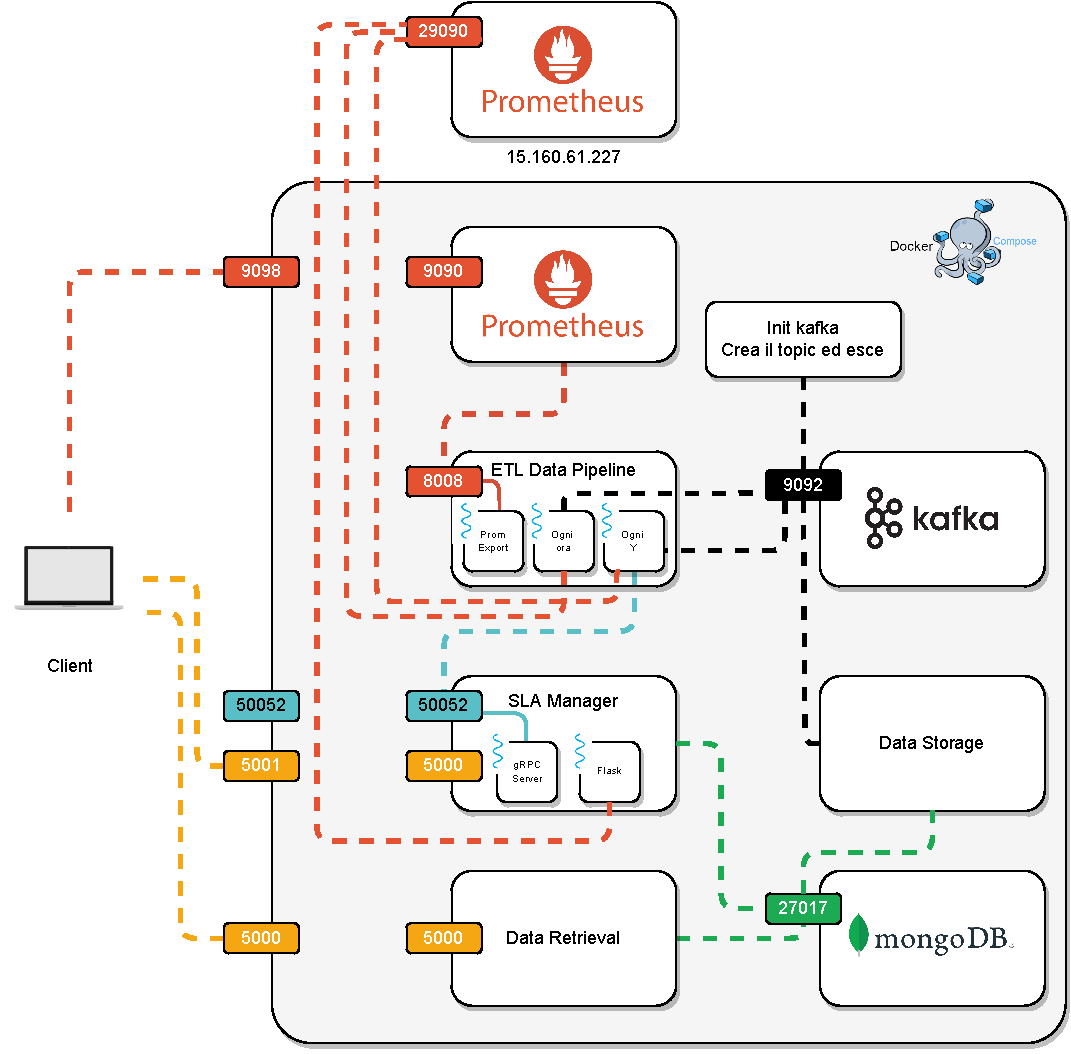
\includegraphics[width=\textwidth]{img/Architettura.pdf}
        \caption{Schema architetturale}
        \label{fig:my_label}
    \end{figure}
    È stato realizzato un sistema di monitoraggio di un applicazione. L'applicazione in oggetto espone le metriche da monitorare mediante un server Prometheus già esistente e raggiungibile all'indirizzo \textit{151.160.61.227:29090}. Per perseguire l'obiettivo vengono realizzati i microservizi descritti a seguire. Per il deploy del sistema si è utilizzato un \textbf{Docker Compose}. È stata effettuata anche una prova di deployment tramite l'orchestratore di container \textbf{Kubernetes}.
    \subsection{ETL Data Pipeline}
    Microservizio che si occupa di Estrarre (\textit{Extract}), Trasformare (\textit{Transform}) e Caricare (\textit{Load}) i dati esposti da Prometheus.  È composto da tre loop che eseguono in parallelo mediante thread:
        \begin{itemize}
            \item Il primo che viene schedulato ogni 2 minuti e si occupa, dopo aver ottenuto i dati dal Prometheus:
            \begin{itemize}
                \item di calcolare i valori massimo, medio, minimo e la deviazione standard per ogni metrica nelle ultime 1, 3 e 12 ore.
                \item di chiedere il set di metriche che compongono l'SLA set all'SLA manager tramite gRPC, disponibile alla porta \textit{50052} (porta configurabile tramite variabile d'ambiente definita nel file \texttt{.env}, così come tutte le successive citate). È stato scelto di utilizzare gRPC perché utilizza una codifica dei dati più snella rispetto al JSON utilizzato nelle API REST. Per ottenere la semantica At-least-once la richiesta viene iterata finchè non si riceve risposta. La semantica Exactly-once non è richiesta dato che la procedura è idempotente. Una volta ottenuta la risposta dalla chiamata remota, se è stato precedentemente definito il set di metriche, per ogni metrica contenuta, viene computata la predizione dei successivi 10 minuti e calcolati i valori massimo, minimo e medio. Vengono calcolate due predizioni mediante la funzione \textit{ExponentialSmoothing}: la prima considerando il modello additivo e la seconda considerando quello moltiplicativo. Viene poi calcolato l'errore quadratico medio e viene tenuta in considerazione la predizione che minimizza l'errore. L'idea iniziale era quella di effettuare la predizione anche tramite il modello ARIMA e poi eseguire il confronto tra le tre. Per problemi implementativi e di tempo non ci siamo riusciti. 
            \end{itemize}
            Invia i valori calcolati nel topic Kafka \textit{prometheusdata} inviando un messaggio per ogni metrica disponibile in Prometheus. Nel caso di deployment su K8s, kafka è stato configurato in maniera differente per ottenere high availability, vedi \ref{sec:kafka}. Per questo motivo abbiamo deciso di impostare acks=all. 
            
            \item Il secondo, schedulato con periodo di un'ora calcola i metadati delle metriche. Viene calcolata dapprima la stazionarietà mediante l'Augmented Dickey–Fuller test.
            
            Successivamente i valori di autocorrelazione sono calcolati tramite la funzione acf di StatsModels. Vengono mostrati tutti i lags con i relativi valori di autocorrelazione, che con un livello di confidenza superiore al 95\%, abbiano valori di autocorrelazione maggiore di 0. 

            Infine viene calcolato il periodo della stagionalità tramite la trasformata di fourier (FFT). Siamo interessati a trovare la frequenza dove l'FFT ha valore massimo, cosicché invertendo troviamo il periodo.
            Ci siamo accorti che il calore così calcolato non è precisissimo. Abbiamo cercato quindi di migliorare il risultato. L'idea è quella di eseguire la funzione SeasonalDecompose nell'intorno del periodo calcolato in precedenza, e cercare il periodo che minimizzi l'errore residuo. Non siamo riusciti a trovare un algoritmo che, in pochi passi, converga in tutte le condizioni. Per le motivazioni di cui prima non è stato pertanto implementato, è stato comunque lasciato come commento nel codice.
            
            Nel caso in cui ci accorgiamo preventivamente che la serie ha un andamento costante, evitiamo al microservizio di effettuare tutti i calcoli precedentemente citati.
            \item Il terzo è un exporter Prometheus che si occupa di rendere disponibili (sulla porta 8008), ad un secondo server Prometheus interno, le metriche raccolte per monitorare i due loop precedenti. In particolare espone le seguenti metriche:
                \begin{itemize}
                    \item etl\_executiontime\_<x>h: con x $\in$ [1, 2, 12]. Per ogni metrica viene calcolato il tempo di esecuzione per calcolare i dati di aggregazione (min, max, avg, dev\_std) nelle ultime x ore;
                    \item etl\_executiontime\_metadata: monitora il tempo di esecuzione speso per calcolare i metadati (stazionarietà, stagionalità, autocorrelazione);
                    \item etl\_executiontime\_prediction: monitora il tempo impiegato per: l'allenamento dei modello predittivi (ExponentialSmoothing additivo e moltiplicativo), la predizione e il confronto degli errori per scegliere il modello più adatto;
                \end{itemize}
            Ognuna delle metriche precedenti contiene una label (metric\_name) usata per distinguere il tempo di esecuzione delle varie funzionalità per ogni metrica.
        \end{itemize}    
    \subsection{Data Storage}
    Microservizio che si occupa di eseguire un polling continuo sul topic kafka \textit{prometheusdata}.
    Per ogni messaggio ricevuto viene effettuato un upsert del documento, identificato mediante nome e labels della metrica, contenuto nel MongoDB.
    \subsubsection{Gestione errori}
        È stato disattivato il commit automatico della lettura per far si che il messaggio consumato venga contrassegnato tale solo nel momento in cui si è sicuri che l'operazione nel database sia andata a buon fine. Nel caso in cui il database non fosse disponibile si ritenta, in seguito, ad effettuare l'operazione.
    
        Durante la sottoscrizione al topic, nel caso in cui venissero riscontrati errori \textit{retriable}, procediamo ad eseguire l'operazione dopo una piccola attesa. Il programma finisce in modo anomalo altrimenti.
    
        Per far si che il topic sia già stato creato nel broker Kafka, il docker contenente il microservizio, viene avviato solo dopo che un altro container (Init Kafka vedi \ref{sec:init_kafka}) abbia finito la propria esecuzione con successo.
    \subsection{Init Kafka}\label{sec:init_kafka}
    Microservizio che si occupa semplicemente di creare, se non esiste, il topic prometheusdata. Una volta che il topic è stato creato con successo, il docker compose si occupa di avviare tutti i container dipendenti (Data Storage, ETL Data Pipeline). Questo microservizio, nel deployment su K8s, è stato sostituito da un Init Container nel pod ETL.
    
    \subsection{Data Retrieval}
    Microservizio che esegue un'applicativo Flask ed espone le API REST descritte in \ref{api:data_retrieval} sulla porta \textit{5000}. Si occupa di recuperare le informazioni presenti nel database MongoDB e mostarle all'utente.
    
    \subsection{SLA Manager}
    Microservizio che in due thread separati esegue un'applicazione Flask esponendo le API descritte in \ref{api:sla_manager} e un server gRPC per la comunicazione con l'ETL Data Pipeline.
    In fase di definizione dell'SLA set è necessario inserire una lista di 5 metriche per ognuna delle quali si deve definire un range di valori ammessi specificando massimo e minimo e il tempo, espresso in minuti, dopo il quale se la metrica esce dal range dei valori ammessi scatta l'allarme.
    \subsection{Ulteriori microservizi}
        \subsubsection{MongoDB} Istanza di un database MongoDB per la persistenza dell'SLA set e la memorizzazione dei dati ottenuti dal Prometheus. È stato scelto MongoDB perché è un database \textit{schemaless}, caratteristica che ha fatto comodo dal momento che alcuni dati hanno una struttura differente (es. label delle metriche).
        \subsubsection{Prometheus} Server Prometheus interno per il monitoraggio dei tempi di esecuzione dell'ETL Data Pipeline raggiungibile dalla porta \textit{9098}.
        \subsubsection{Kafka e Zookeeper} \label{sec:kafka}
            Kafka fa uso di Zookeeper per l'elezione del controller all'interno di un cluster. Questo è importante, non tanto nel deploy effettuato con il compose (in quanto abbiamo un solo broker), quanto nel deploy su Kubernetes. In quest'ultimo abbiamo deciso di realizzare un cluster composto da 3 broker. Il topic kafka è stato creato quattro partizioni e replication factor pari a 3, così da ottenere \textit{high availability} e scalabilità.
    





        
\section{Istruzioni}
Prerequisiti: 
    \begin{itemize}
        \item Docker
        \item Postman (opzionale)
    \end{itemize}
I comandi descritti a seguire vanno lanciati dalla directory principale del progetto.
\subsection{Docker compose}
Per procedere con l'esecuzione del sistema è sufficiente eseguire il comando:  
\begin{minted}{bash}
  $ docker compose up
\end{minted}
Durante la prima esecuzione del comando verrà eseguito il pull delle immagini pubbliche preesistenti e il build delle immagini create ad hoc.
\subsection{Kubernetes}
\subsubsection{Build delle immagini}
Se è stato già eseguito il docker compose saltare questo passaggio. Altrimenti per eseguire il build delle immagini:
\begin{minted}{bash}
  $ docker compose build
\end{minted}
dal momento che le immagini utilizzate sono le stesse.
\subsubsection{Deployment}
Per il depolyment, utilizzando un qualsiasi cluster Kubernetes (anche composto da un solo nodo come ad esempio minikube, kind o Docker Desktop), applicare tutti i file di configurazione yaml contenuti nella cartella Kubernetes. Dalla directory del progetto:
\begin{minted}{bash}
  $ kubectl apply -f Kubernetes -R
\end{minted}
\subsection{Caricamento SLA set}
Ulteriore passo per provare le API REST e quello di definire l'SLA set seguendo una delle due procedure illustrate a seguire.
\subsubsection{Postman}
Andare su \texttt{File} > \texttt{Import...}

Nella finestra che si apre andare nel tab \texttt{File} > \texttt{Choose Files} e selezionare il file \texttt{DSBD.postman\_collection.json}. Accettarsi che  le spunte siano selezionate e cliccare su \texttt{Import}.

Si avranno a disposizione tutte le API rese disponibili dai microservizi. Selezionare \texttt{SLA Manager > CREATE/UPDATE dell'SLA}
\subsubsection{Curl}
Per eseguire manualmente la creazione dell'SLA set eseguire il comando curl:
\begin{minted}{bash}
curl --location --request PUT 'http://localhost:5001/slaset' \
--header "Content-Type: application/json" -d @sla_set.json 
\end{minted}
\newpage
\appendix
\section{API implementate}
\subsection{Data Retrieval}
API disponibili sulla porta \textit{5000} dell'host che esegue il Docker Compose. \textit{31000} nel caso di Kubernetes.
\label{api:data_retrieval}
    \subsubsection{QUERY di tutte le metriche disponibili in Prometheus}
    \begin{apiRoute}{get}{/metrics}{fornisce la lista delle metriche disponibili nel database}
    	\begin{routeResponse}{application/json}
    		\begin{routeResponseItem}{200}{OK}
    			\begin{routeResponseItemBody}
[
    {
        "_id": {
            "$oid": "63d00c1a40f34de7a72b4168"
        },
        "name": {
            "__name__": "node_filesystem_avail_bytes",
            "device": "/dev/sda2",
            "fstype": "ext4",
            "instance": "node-exporter:9100",
            "job": "host",
            "mountpoint": "/"
        }
    },
    {
        "_id": {
            "$oid": "63d00c1a40f34de7a72b416e"
        },
        "name": {
            "__name__": "node_filesystem_avail_bytes",
            "device": "tmpfs",
            "fstype": "tmpfs",
            "instance": "node-exporter:9100",
            "job": "host",
            "mountpoint": "/run"
        }
    }
    ...
]
        
    			\end{routeResponseItemBody}
    		\end{routeResponseItem}
    		\begin{routeResponseItem}{504}{error: Gateway Timeout}
    			\begin{routeResponseItemBody}
DB not available
    			\end{routeResponseItemBody}
    		\end{routeResponseItem}
    	\end{routeResponse}
    	
    \end{apiRoute}
\subsubsection{QUERY dei metadata}
    
    \begin{apiRoute}{get}{/metrics/\{id\}/metadata}{}
    	
    	\begin{routeParameter}
    		\routeParamItem{id}{metric id}
    	\end{routeParameter}
    	\begin{routeResponse}{application/json}
    		\begin{routeResponseItem}{200}{OK}
    			\begin{routeResponseItemBody}
{
    "metadata": {
        "stationarity": {
            "stationary": false,
            "p_value": 0.19978974023640284
        },
        "autocorrelation": {
            "0": 1.0,
            "1": 0.997171498017174,
            "2": 0.9942726635385408,
            "7": 0.9800894708048338,
            "9": 0.9745687748924085,
            "11": 0.9690954658172681,
            "22": 0.9393540767588636,
            "27": 0.9262209581943193,
            "31": 0.9158247688017431,
        },
        "seasonality": {
            "add": {
                "period": 1440,
                "error": 231207587.304691
            },
            "mul": {
                "period": 1440,
                "error": 0.019785233109260503
            }
        }
    }
}
    			\end{routeResponseItemBody}
    		\end{routeResponseItem}
                \begin{routeResponseItem}{504}{error: Gateway Timeout}
    			\begin{routeResponseItemBody}
DB not available
    			\end{routeResponseItemBody}
    		\end{routeResponseItem}
    		\begin{routeResponseItem}{400}{error: Bad Request}
    			\begin{routeResponseItemBody}
Invalid metric id or no metadata found for given id
    			\end{routeResponseItemBody}
    		\end{routeResponseItem}
    	\end{routeResponse}
    	
    \end{apiRoute}

\subsubsection{QUERY dei valori max, min, avg, dev\_std per le ultime 1,3,12 ore}
    \begin{apiRoute}{get}{/metrics/\{id\}/values}{Ritorna i valori di aggregazione massimo, minimo, media e deviazione standard calcolati per i campioni delle ultime 1, 3 e 12 ore della metrica di cui viene passato l'identificativo}
    	
    	\begin{routeParameter}
    		\routeParamItem{id}{metric id}
    	\end{routeParameter}
    	\begin{routeResponse}{application/json}
    		\begin{routeResponseItem}{200}{OK}
    			\begin{routeResponseItemBody}
{
    "values": {
        "1h": {
            "min": 10449256448.0,
            "max": 10617593856.0,
            "avg": 10523682133.333334,
            "std_dev": 43891016.15905848
        },
        "3h": {
            "min": 10449256448.0,
            "max": 10961149952.0,
            "avg": 10679585609.955555,
            "std_dev": 137401532.7018694
        },
        "12h": {
            "min": 10449256448.0,
            "max": 12566388736.0,
            "avg": 11467336510.577778,
            "std_dev": 627568959.1682327
        }
    }
}
    			\end{routeResponseItemBody}
    		\end{routeResponseItem}
                \begin{routeResponseItem}{504}{error: Gateway Timeout}
    			\begin{routeResponseItemBody}
DB not available
    			\end{routeResponseItemBody}
    		\end{routeResponseItem}
    		\begin{routeResponseItem}{400}{error: Bad Request}
    			\begin{routeResponseItemBody}
Invalid metric id or no values found for given id
    			\end{routeResponseItemBody}
    		\end{routeResponseItem}
    	\end{routeResponse}
    	
    \end{apiRoute}
\newpage
\subsubsection{QUERY dei valori predetti}
    \begin{apiRoute}{get}{/metrics/\{id\}/prediction}{Ritorna il valore massimo, minimo e medio dei valori predetti nonché questi ultimi in formato csv e il root mean square error della previsione con errore minore}
    	
    	\begin{routeParameter}
    		\routeParamItem{id}{metric id}
    	\end{routeParameter}
    	\begin{routeResponse}{application/json}
    		\begin{routeResponseItem}{200}{OK}
    			\begin{routeResponseItemBody}
{
    "prediction": {
        "min": 10417014788.917332,
        "max": 10445513497.009878,
        "avg": 10432558690.63635,
        "values": ",0\n2023-01-25 20:02:00,10432568427.843391\n2023-01-25 20:03:00,10429244157.682781\n2023-01-25 20:04:00,10445513497.009878\n2023-01-25 20:05:00,10437680451.247105\n2023-01-25 20:06:00,10434635919.70584\n2023-01-25 20:07:00,10439117885.560318\n2023-01-25 20:08:00,10430276782.411537\n2023-01-25 20:09:00,10433978218.499474\n2023-01-25 20:10:00,10425556777.48585\n2023-01-25 20:11:00,10417014788.917332\n",
        "rmse": 118084489.44144112
    }
}
    			\end{routeResponseItemBody}
    		\end{routeResponseItem}
                \begin{routeResponseItem}{504}{error: Gateway Timeout}
    			\begin{routeResponseItemBody}
DB not available
    			\end{routeResponseItemBody}
    		\end{routeResponseItem}
    		\begin{routeResponseItem}{400}{error: Bad Request}
    			\begin{routeResponseItemBody}
Invalid metric id or no prediction found for given id
    			\end{routeResponseItemBody}
    		\end{routeResponseItem}
    	\end{routeResponse}
    	
    \end{apiRoute}
\newpage
\subsection{SLA Manager}
    \subsubsection{API REST}
    API disponibili sulla porta \textit{5001} dell'host che esegue il Docker Compose. \textit{31001} nel caso di Kubernetes.
    \label{api:sla_manager}
        \paragraph{QUERY get SLA Set}
    \begin{apiRoute}{get}{/slaset}{fornisce l'SLA set}
    	\begin{routeParameter}
    		\noRouteParameter{no parameter}
    	\end{routeParameter}
    	\begin{routeResponse}{application/json}
    		\begin{routeResponseItem}{200}{OK}
    			\begin{routeResponseItemBody}
[
    {
        "_id": {
            "$oid": "63d1206fd124ee3315cfe886"
        },
        "name": {
            "__name__": "node_filesystem_avail_bytes",
            "device": "tmpfs",
            "fstype": "tmpfs",
            "instance": "node-exporter:9100",
            "job": "host",
            "mountpoint": "/run"
        },
        "range": {
            "min": 3289686016,
            "max": 3290595328
        },
        "for": 1
    },
    ...
]      
    			\end{routeResponseItemBody}
    		\end{routeResponseItem}
    		\begin{routeResponseItem}{504}{error: Gateway Timeout}
    			\begin{routeResponseItemBody}
DB not available
    			\end{routeResponseItemBody}
    		\end{routeResponseItem}
    	\end{routeResponse}
    \end{apiRoute}
\newpage
\paragraph{CREATE/UPDATE dell'SLA }
    \begin{apiRoute}{put}{/slaset}{aggiorna o crea l'SLA set}
    	\begin{routeRequest}{application/json}
    		\begin{routeRequestBody}
[ 
    {     
        "name": {
            "__name__": "node_filesystem_avail_bytes",
            ... 
            "mountpoint": "/run"
        },
        "range": { "min": 328, "max": 3290595},
        "for": 5
    },
    ...
]
    		\end{routeRequestBody}
    	\end{routeRequest}
    	\begin{routeResponse}{text/html}
    		\begin{routeResponseItem}{200}{OK}
    			\begin{routeResponseItemBody}
SLA set updated
    			\end{routeResponseItemBody}
    		\end{routeResponseItem}
                \begin{routeResponseItem}{201}{Created}
    			\begin{routeResponseItemBody}
SLA set created
    			\end{routeResponseItemBody}
    		\end{routeResponseItem}              
                \begin{routeResponseItem}{400}{error: Bad request}
    			\begin{routeResponseItemBody}
SLA set must consist of 5 metrics. {} provided
- The metric {} does not exists;
- Minimum value of range not provided for {};
- Maximum value of range not provided for {};
- Invalid range provided [minimum given value ({}) is greater than maximum one ({})] for {};
- Range not provided for {};
- Invalid duration (for key) provided for {};
- Duration (for key) not provided for {};
    			\end{routeResponseItemBody}
    		\end{routeResponseItem}
                \begin{routeResponseItem}{500}{error: Internal Server Error}
    			\begin{routeResponseItemBody}
Error on db
    			\end{routeResponseItemBody}
    		\end{routeResponseItem}
                \begin{routeResponseItem}{504}{error: Gateway Timeout}
    			\begin{routeResponseItemBody}
DB not available
    			\end{routeResponseItemBody}
    		\end{routeResponseItem}
    	\end{routeResponse}
    \end{apiRoute}



\paragraph{QUERY dello stato dell’SLA}
\begin{apiRoute}{get}{/status}{ritorna lo stato dell'SLA. Il campo \textbf{description} può essere (in funzione dello stato): 
            \begin{itemize}
                \item \textbf{inactive}: Actual value [\{\}] in (\{\}, \{\})
                \item \textbf{pending}: Service level agreement violated for \{\}/\{\} min (\{\%\}), last three values [\{\},\{\},\{\}] not in (\{\}, \{\})
                \item \textbf{firing}: Service level agreement violated for more than \{\} min, last three values \{\}, allowed range: (\{\}, \{\})
            \end{itemize}
        }
    	\begin{routeParameter}
    		\noRouteParameter{no parameter}
    	\end{routeParameter}
    	\begin{routeResponse}{application/json}
    		\begin{routeResponseItem}{200}{OK}
    			\begin{routeResponseItemBody}
[
    {
        "name": {
            "device": "tmpfs",
            "fstype": "tmpfs",
            "instance": "node-exporter:9100",
            "job": "host",
            "mountpoint": "/run"
        },
        "status": "inactive",
        "description": "Actual value [3289706496.0] in (3289686016, 3290595328)",
        "last-values": [
            3289759744.0,
            3289731072.0,
            3289706496.0
        ]
    },
    ...
]     
    			\end{routeResponseItemBody}
    		\end{routeResponseItem}
    		\begin{routeResponseItem}{504}{error: Gateway Timeout}
    			\begin{routeResponseItemBody}
DB not available
    			\end{routeResponseItemBody}
    		\end{routeResponseItem}
    	\end{routeResponse}
    	
    \end{apiRoute}

\newpage
\paragraph{QUERY del numero di violazioni nelle ultime 1, 3, 12 ore}
    \begin{apiRoute}{get}{/violations}{ritorna il numero di violazioni nelle ultime 1, 3 e 12 ore. Ritorna inoltre per ognuna delle fasce il tempo totale di violazione, e una lista di tutte le violazioni nelle ultime 12 ore}
    	\begin{routeResponse}{application/json}
    		\begin{routeResponseItem}{200}{OK}
    			\begin{routeResponseItemBody}
[
    {
        "name": {
            "device": "/dev/vda1",
            "fstype": "ext4",
            "instance": "node_exporter:9100",
            "job": "node",
            "mountpoint": "/etc/resolv.conf"
        },
        "1h": {
            "n": 1, "time": 60.0
        },
        "3h": {
            "n": 1, "time": 76.0
        },
        "12h": {
            "n": 1, "time": 76.0
        },
        "violation_list": [
            {
                "start_time": "2023-01-23 10:14:24",
                "end_time": "2023-01-23 11:30:24",
                "duration": 76.0,
                "avg_value": 39738415265.68421,
                "max_value": 40542871552.0,
                "min_value": 37894434816.0
            }
        ]
    }
    ...
]  
    			\end{routeResponseItemBody}
    		\end{routeResponseItem}
                \begin{routeResponseItem}{400}{error: Bad request}
    			\begin{routeResponseItemBody}
SLA set not defined
    			\end{routeResponseItemBody}
    		\end{routeResponseItem}
    		\begin{routeResponseItem}{504}{error: Gateway Timeout}
    			\begin{routeResponseItemBody}
DB not available
    			\end{routeResponseItemBody}
    		\end{routeResponseItem}
    	\end{routeResponse}
    	
    \end{apiRoute}

\paragraph{QUERY su possibili violazioni future dell’SLA}
    \begin{apiRoute}{get}{/future-violations}{Ritorna la lista delle possibili violazioni nei futuri 10 minuti, per ogni metrica appartenente al set. Per ogni violazione viene riportato: il timestamp di inizio e fine violazione, la durata, i valori max, avg e min e una descrizione che puo essere: 
    \begin{itemize}[nosep]
        %\setlength\itemsep{0em}
        \item Was already firing, continuing firing
        \item Was pending, will fire
        \item Will fire
        \item Will be pending      
    \end{itemize} }
    	\begin{routeResponse}{application/json}
    		\begin{routeResponseItem}{200}{OK}
    			\begin{routeResponseItemBody}
[
    {
        "name": { ... },
        "error": "Prediction not available"
    },
    ...,
    {
        "name": { ... },
        "violations": [
            {
               "start_time": "2023-01-25 12:12:53",
               "end_time": "2023-01-25 12:24:00",
               "duration": 12,
               "description": "Was pending, will fire",
               "avg_value": 11728352970.995926,
               "max_value": 11757084672.0,
               "min_value": 11704975159.982656
            }
        ],
        "prediction_rmse": 118084489.44144112
    }
]
    			\end{routeResponseItemBody}
    		\end{routeResponseItem}
                \begin{routeResponseItem}{504}{error: Gateway Timeout}
    			\begin{routeResponseItemBody}
DB not available
    			\end{routeResponseItemBody}
    		\end{routeResponseItem}
    		\begin{routeResponseItem}{400}{error: Bad Request}
    			\begin{routeResponseItemBody}
SLA set not defined
    			\end{routeResponseItemBody}
    		\end{routeResponseItem}
    	\end{routeResponse}
    	
    \end{apiRoute}
    
    \subsubsection{gRPC}
        \SetProtoColorsBlueish
        \lstinputlisting[language=protobuf2, style=protobuf,caption={Protobuf API gRPC.}]{gRPC/sla.proto}

\end{document}



